\documentclass[a4paper, 11pt]{article}

\usepackage[utf8]{inputenc}

\usepackage[T1]{fontenc}

\usepackage[english]{babel}

\usepackage{graphicx}

\usepackage{multicol}

\usepackage{floatrow}

\usepackage[margin = 1in]{geometry}

\usepackage{float}

\usepackage[hidelinks, urlcolor=cyan]{hyperref}

\usepackage{url}

\usepackage{natbib}

\bibliographystyle{abbrvnat}
\setcitestyle{authoryear,open={(},close={)}}

\usepackage{csquotes}

\usepackage{fancyhdr}

\usepackage{lipsum}

\usepackage{adjustbox}
\usepackage{rotating}
\usepackage[table,xcdraw]{xcolor}

%\addbibresource{references.bib}

\title{\Large BINF-F401 Project \\
\huge Analysis of the morphological clusters from heart and there associations with clinical and transcriptomic data.}


\author{
	Draguet Simon
	\and
	Godin Maximilien
	\and
	Guyot Léopold
	}

\date{\today}

\begin{document}

\pagestyle{fancy}
\setlength{\headheight}{32.3pt}
\fancyhead{}\fancyfoot{}
\fancyhead[L]{
\includegraphics[scale = 0.05]{figures/LOGO_Universite _libre_bruxelles.png}}
\fancyhead[R]{Analysis of the morphological clusters from heart}
\fancyfoot[R]{\thepage}

\maketitle

\begin{multicols}{2}

\section{Introduction}
R \citep{R:2024}

\section{Exploration of  clinical variables}
Description des variables .....  

\subsection{Distribution of the variables}

\begin{scriptsize}	
	
	\textbf{Associated script : \href{https://github.com/leopoldguyot/BINF-F401-Project/*}{.R}}
\end{scriptsize}

By examining the clinical variables through histograms, we can visualize their distribution. Most of the continuous variables do not seem to follow a normal distribution. For instance, the variable AGE appears to be asymmetric, exhibiting a right skew (fig X).
To now if the continuous variable were normally distributed, we used a Shapiro-Wilk test. The results showed that AGE, HGHT, BMI, TRISCHD all had p-value under 5\%, leading us to reject the null hypothesis, which say that the sample is drawn form a normally distributed population. However, for WGHT, it was higher than 5 , so we didn’t reject the null hypothesis (table X ) . 

To do further analysis, we need them to be normally distributed. We tried to apply various transformations like log, square root, square. Only the square transformation successfully normalized the AGE sample. 
Because we needed it to work on all the continuous variable, we finally chose to use the rank-based inverse normal transformation (INT). that first convert the variable into ranks, then map it to a normal distribution. 

$ Y^t_{i}=  \Phi^{-1}(r-C/N-2C+1) $

where $r_i$ is the ordinary rank of the $_ith$ case among the N observations and $\Phi^{-1}$ denotes the standard normal quantile (or probit) function.For the value of C we use C=3/8 \citep{beasley2009rank}.

If we look at the discrete variable, we can see that we don't have a balanced distribution. For example, for the variable AGE, there are more than twice as many males as females (fig x). For DTHHRDY, we can observe that most of the deaths occurred in ventilator cases (fig x). When conducting analysis, it's essential to keep these observations in mind as they can significantly influence the interpretation. 

\subsection{Correlations between the clinical variables}

Principal Component Analysis (PCA) is a method of determining individual profiles and linear relationships between variables, based on correlation coefficients. The various graphs produced by a PCA, notably the correlation circle, are therefore a good way of illustrating the links between different quantitative variables, and getting a general idea of these links. Nevertheless, the data we are considering here are also partly qualitative. It is therefore preferable to turn to a Factor Analysis of Mixed Data, i.e. an analysis that applies a PCA to quantitative variables and a Multiple Correspondence Analysis to qualitative variables. The various dimensions defined by this method can be used to characterize all the variables. The FAMD() function in the FactoMineR package was used, with the argument allowing the creation of a series of graphs.

\begin{figure}[H]
	\centering
	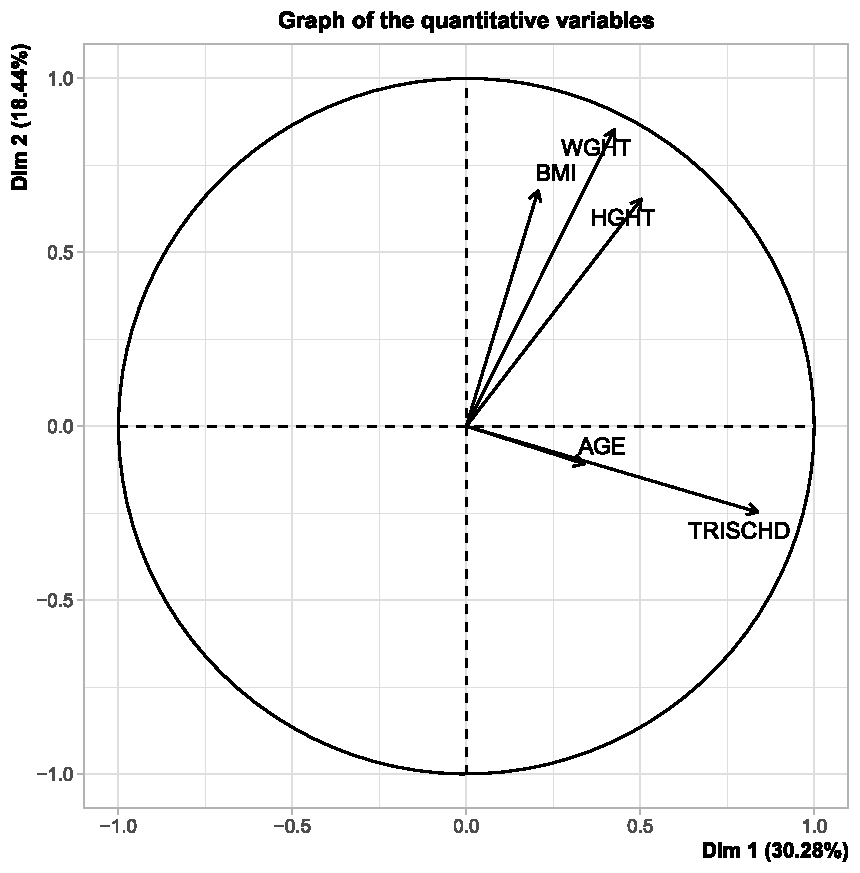
\includegraphics[width=\columnwidth]{figures/clinical_correlation_plots/all_quant_Dim2}
	\caption{Correlation circle of the continuous variables}
	\label{fig:corCircle}
\end{figure}

\begin{figure}[H]
	\centering
	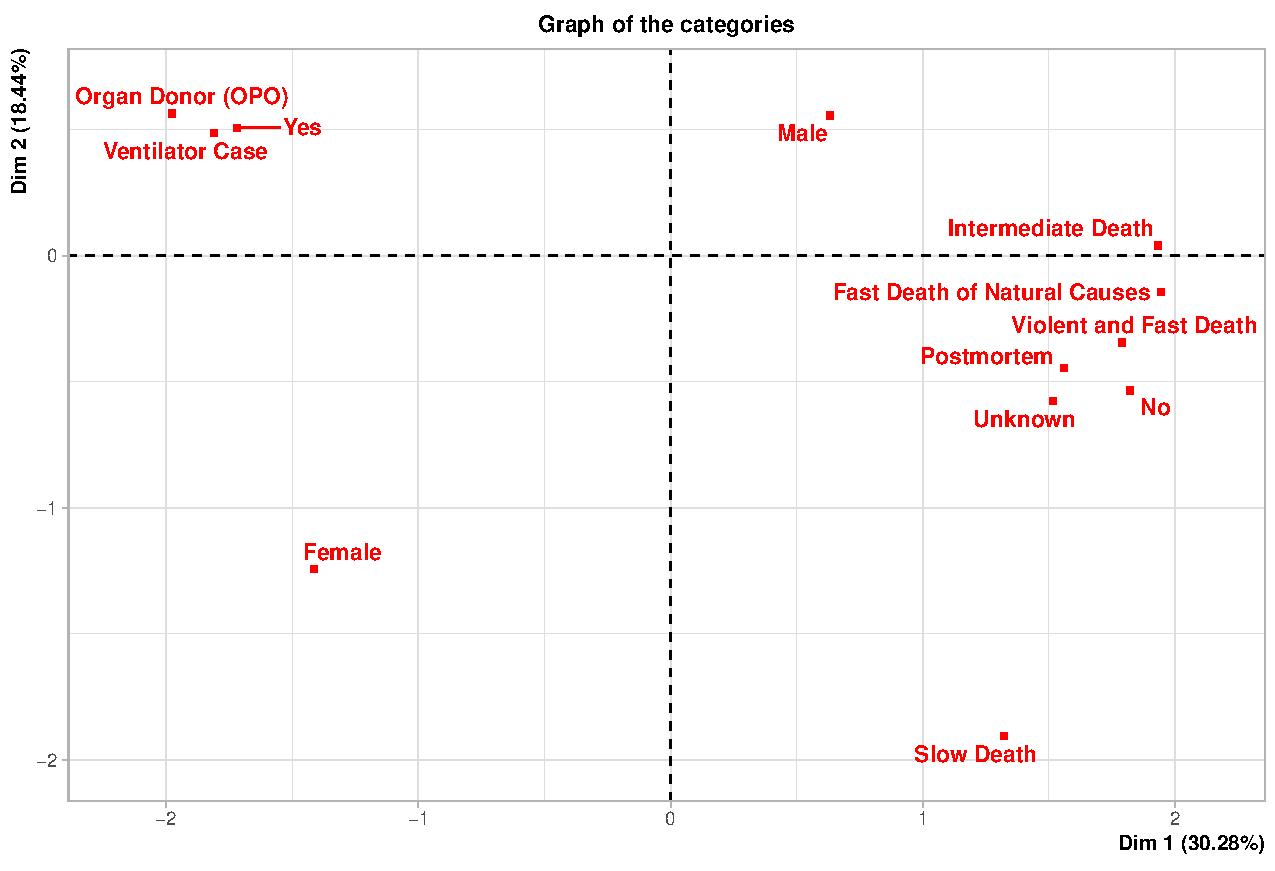
\includegraphics[width=\columnwidth]{figures/clinical_correlation_plots/all_categ_Dim}
	\caption{Level maps of all the different categories in the qualitative variables}
	\label{fig:lvlMap}
\end{figure}

The correlation circle allows us to represent quantitative variables according to the relationships they might have with each other, and the degree of explanation of these variables provided by the chosen dimensions. 
In this case, the two dimensions represented together explain only 48.72\% of the data, suggesting a certain complexity. 
This graph shows some correlation between the variables height (HGHT), weight (WGHT) and body mass index (BMI), which is not surprising given that taller people tend to be heavier, and also given that BMI is a function of height and weight. 
There also appears to be a correlation between age (AGE) and ischemic time (TRISCHD), i.e. the time between an individual's death and organ removal. 
This last observation is more difficult to explain intuitively. 
We can, however, point out that the variable AGE is weakly explained by the first two dimensions chosen, since its vector is close to the origin. 
This indicates that this possible correlation may not be significant, since by considering other dimensions, the vectors could be significantly far apart.

In contrast to the correlation circle, the level map represents the different categories or levels of categorical variables. 
We can already see that gender is close to different clusters. 
It would seem that there is a correlation between gender and type of death in these data, given that women seem to be more prone to ventilatory problems than men, which would explain the presence of a respirator before the person's death (Yes). 
It also appears that women are more likely than men to be organ donors. This graph therefore shows a certain correlation between gender and organ donation, type of death, but also between type of death and the presence or absence of a respiratory system prior to death.

Although these graphs illustrate the presence of possible correlations, they do not give any indication of their intensity, as they are not quantified. 
This quantification of correlation is particularly complex, as there is no correlation coefficient that can be applied to either quantitative or qualitative variables, or between these two types of variable. 
It was therefore decided to use different coefficients depending on the type of comparison, although this choice does not allow all correlations to be compared with each other. 
Correlations between quantitative variables were established using the cor() function with Spearman's method. 
This correlation was chosen because it does not require normally distributed variables, which is not the case for most of the variables considered. 
This coefficient is the only one to consider negative correlations.
Cramer's V was used to determine correlations between categorical variables, a coefficient based on the Chi-square statistic, and which is non-parametric. 
This correlation was calculated using the cramerV() function in the rcompanion package, with a bias correction given that this test tends to overestimate the relationships between categorical variables.
Logistic regression is used to determine the correlation between a quantitative variable and a binomial categorical variable, in this case gender and cohort. 
Finally, Cramer's V is applied to the H statistic of the Kruskall-Willis test between categorical and quantitative variables, as this statistic is the Kruskall-Willis chi-square. This application simply involves calculating the square root of the H statistic divided by the number of observations, the H statistic coming from the kruskall.willis() function.

\begin{figure}[H]
	\centering
	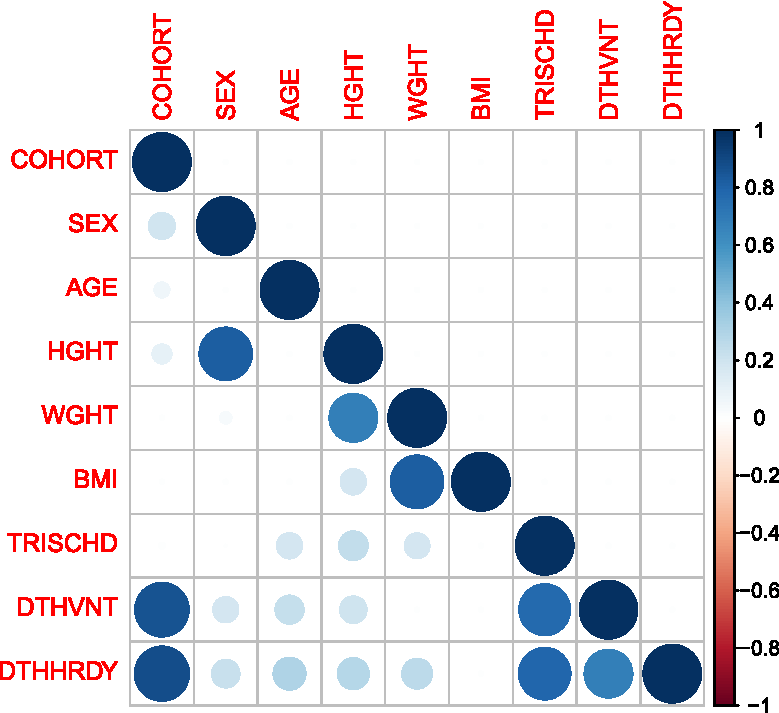
\includegraphics[width=\columnwidth]{figures/clinical_correlation_plots/corrected_allCorrelations2}
	\caption{Correlation matrix of all the variables}
	\label{fig:allCor}
\end{figure}

Looking at all the results together, we can see that there is a significant correlation between gender and height, which can simply be explained by the fact that men are generally taller than women. 
The correlation between height and weight, as well as between weight and BMI, can be explained as described above. 
Nevertheless, the absence of any significant correlation between height and BMI is rather odd given that the BMI calculation takes into account both height and weight, and that the correlation circle has positioned the corresponding vectors relatively close to each other. 
There is also a correlation between cohort and both type of death (DTHHRDY) and use of artificial ventilation before death (DTHVNT). 
There is a certain logic behind these correlations: the cohort variable divides people into organ donors and postmortem donors, i.e. victims of brain or cardiac death, thus depending on the type of death, but we can also consider that people with brain death are generally assisted with artificial ventilation before death. 
There also seems to be a correlation between the time between the individual's death and the removal of his or her organs and the type of death, but also the presence of a ventilatory apparatus. 
Finally, DTHVNT and DTHHRDY are also correlated.

\begin{table*}[t]
\footnotesize
\makebox[\linewidth]{
\begin{tabular}{|c|c c|c|c c|c c|c c|c|c c|c|cc|}
\cline{2-8}
    \hline & \multicolumn{2}{c|}{\rotatebox{90}{AGE}} & \rotatebox{90}{SEX} & \multicolumn{2}{c|}{\rotatebox{90}{HGHT}} & \multicolumn{2}{c|}{\rotatebox{90}{WGHT}} & \multicolumn{2}{c|}{\rotatebox{90}{BMI}} & \rotatebox{90}{COHORT} & \multicolumn{2}{c|}{\rotatebox{90}{TRISCHD}} & \rotatebox{90}{DTHVNT} & \multicolumn{2}{c|}{\rotatebox{90}{DTHHRDY}} \\
    \hline 
\rotatebox{90}{Cluster} &
  \rotatebox{90}{Normalized} &
  \rotatebox{90}{Categorical (56+ vs -56)} &
  \rotatebox{90}{Female vs Male} &
  \rotatebox{90}{Normalized} &
  \rotatebox{90}{Categorical (71+ vs -71)} &
  \rotatebox{90}{Normalized} &
  \rotatebox{90}{Categorical (181+ vs -181)} &
  \rotatebox{90}{Normalized} &
  \rotatebox{90}{Categorical (28+ vs -28)} &
  \rotatebox{90}{PostMortem vs OrganDonor} &
  \rotatebox{90}{Normalized} &
  \rotatebox{90}{Categorical (50+ vs -50)} &
  \rotatebox{90}{Yes vs No} &
  \rotatebox{90}{Intermediate vs Slow} &
  \rotatebox{90}{Fast vs Slow} \\
  \hline
0 &  & \cellcolor[HTML]{FDFF89}1,22 & \cellcolor[HTML]{B4F5F2}-1,26 &  &  &  &  &  &  & \cellcolor[HTML]{FDFF89}1,98 &  & \cellcolor[HTML]{FDFF89}1,78 & \cellcolor[HTML]{B4F5F2}-1,49 & \cellcolor[HTML]{FDFF89}2,10 & \cellcolor[HTML]{FDFF89}2,00 \\
1 &  &  &  &  &  &  &  &  &  &  &  &  &  &  &  \\
2 &  & \cellcolor[HTML]{FDFF89}1,87 & \cellcolor[HTML]{B4F5F2}-1,99 &  &  &  & \cellcolor[HTML]{FDFF89}1,15 &  & \cellcolor[HTML]{FDFF89}1,70 & \cellcolor[HTML]{FDFF89}2,46 &  & \cellcolor[HTML]{FDFF89}2,36 & \cellcolor[HTML]{B4F5F2}-2,38 & \cellcolor[HTML]{FDFF89}1,71 & \cellcolor[HTML]{FFC702}2,85 \\
3 &  &  &  &  &  &  &  &  &  & \cellcolor[HTML]{FDFF89}1,24 &  &  &  &  &  \\
4 &  &  &  &  &  &  &  &  &  &  &  &  &  &  &  \\
5 &  &  &  &  &  &  &  &  &  & \cellcolor[HTML]{FDFF89}1,55 &  & \cellcolor[HTML]{FDFF89}1,19 & \cellcolor[HTML]{B4F5F2}-1,41 &  &  \\
6 &  &  & \cellcolor[HTML]{FDFF89}1,70 & \cellcolor[HTML]{B4F5F2}-1,02 & \cellcolor[HTML]{B4F5F2}-2,32 &  &  &  &  & \cellcolor[HTML]{6F94FF}-5,33 &  & \cellcolor[HTML]{6F94FF}-5,91 & \cellcolor[HTML]{F56B00}6,27 & \cellcolor[HTML]{6F94FF}-6,34 & \cellcolor[HTML]{6F94FF}-5,90 \\
7 &  &  &  &  &  &  &  &  &  & \cellcolor[HTML]{B4F5F2}-1,10 &  &  &  &  &  \\
8 &  &  & \cellcolor[HTML]{FDFF89}1,03 &  &  &  &  &  &  & \cellcolor[HTML]{B4F5F2}-2,31 &  & \cellcolor[HTML]{B4F5F2}-2,02 & \cellcolor[HTML]{FDFF89}2,17 & \cellcolor[HTML]{B4F5F2}-2,25 & \cellcolor[HTML]{B4F5F2}-2,02 \\
9 &  &  &  &  &  &  &  &  &  & \cellcolor[HTML]{FDFF89}1,17 &  &  &  &  &  \\
10 &  & \cellcolor[HTML]{B4F5F2}-1,53 & \cellcolor[HTML]{FDFF89}1,07 &  & \cellcolor[HTML]{4AD7FF}-2,69 &  & \cellcolor[HTML]{4AD7FF}-2,60 &  &  & \cellcolor[HTML]{6F94FF}-6,72 & \cellcolor[HTML]{B4F5F2}-1,12 & \cellcolor[HTML]{6F94FF}-6,90 & \cellcolor[HTML]{F56B00}7,35 & \cellcolor[HTML]{6F94FF}-6,41 & \cellcolor[HTML]{6F94FF}-7,12 \\
11 &  &  &  &  &  &  &  &  &  &  &  &  &  &  &  \\
12 &  &  &  &  &  &  &  &  &  & \cellcolor[HTML]{B4F5F2}-1,32 &  &  & \cellcolor[HTML]{FDFF89}1,03 &  &  \\
13 &  &  &  &  &  &  &  &  &  &  &  &  &  &  &  \\
14 &  &  &  &  &  &  &  &  &  & \cellcolor[HTML]{B4F5F2}-1,84 &  & \cellcolor[HTML]{B4F5F2}-1,72 & \cellcolor[HTML]{FDFF89}1,78 & \cellcolor[HTML]{B4F5F2}-1,62 & \cellcolor[HTML]{B4F5F2}-1,58 \\
15 &  &  &  &  &  &  &  &  &  & \cellcolor[HTML]{FDFF89}1,25 &  & \cellcolor[HTML]{FDFF89}1,04 & \cellcolor[HTML]{B4F5F2}-1,03 &  &  \\
16 &  &  &  &  &  &  &  &  &  & \cellcolor[HTML]{FDFF89}1,48 &  & \cellcolor[HTML]{FDFF89}1,19 & \cellcolor[HTML]{B4F5F2}-1,07 & \cellcolor[HTML]{FDFF89}1,41 &  \\
17 &  &  &  &  &  &  &  &  &  & \cellcolor[HTML]{B4F5F2}-1,42 &  &  &  &  & \cellcolor[HTML]{B4F5F2}-1,20 \\
18 &  &  &  &  &  & \cellcolor[HTML]{FFC702}4,40 &  & \cellcolor[HTML]{FFC702}3,12 &  &  & \cellcolor[HTML]{6F94FF}-5,25 &  &  &  &  \\
19 &  &  &  &  &  &  &  &  &  &  &  &  &  &  &  \\
20 &  &  & \cellcolor[HTML]{FDFF89}1,02 &  &  &  &  &  &  & \cellcolor[HTML]{B4F5F2}-2,38 &  & \cellcolor[HTML]{B4F5F2}-2,07 & \cellcolor[HTML]{FDFF89}2,44 & \cellcolor[HTML]{B4F5F2}-2,43 & \cellcolor[HTML]{B4F5F2}-2,26 \\
21 &  &  & \cellcolor[HTML]{B4F5F2}-1,09 &  &  &  &  &  &  & \cellcolor[HTML]{FDFF89}1,83 &  & \cellcolor[HTML]{FDFF89}1,60 & \cellcolor[HTML]{B4F5F2}-1,69 & \cellcolor[HTML]{FDFF89}1,68 & \cellcolor[HTML]{FDFF89}1,73 \\
22 &  &  &  &  &  &  &  &  &  & \cellcolor[HTML]{FDFF89}1,47 &  & \cellcolor[HTML]{FDFF89}1,22 & \cellcolor[HTML]{B4F5F2}-1,26 & \cellcolor[HTML]{FDFF89}1,23 & \cellcolor[HTML]{FDFF89}1,02 \\
23 &  &  & \cellcolor[HTML]{FDFF89}1,28 &  & \cellcolor[HTML]{B4F5F2}-1,56 &  &  &  &  & \cellcolor[HTML]{4AD7FF}-4,53 &  & \cellcolor[HTML]{4AD7FF}-4,22 & \cellcolor[HTML]{F56B00}5,19 & \cellcolor[HTML]{6F94FF}-5,27 & \cellcolor[HTML]{4AD7FF}-4,91 \\
24 &  &  &  &  &  &  &  &  &  & \cellcolor[HTML]{FDFF89}2,19 &  & \cellcolor[HTML]{FDFF89}1,93 & \cellcolor[HTML]{B4F5F2}-1,61 & \cellcolor[HTML]{FDFF89}2,22 & \cellcolor[HTML]{FDFF89}2,09 \\
25 &  &  & \cellcolor[HTML]{FDFF89}1,59 &  & \cellcolor[HTML]{B4F5F2}-1,42 &  &  &  &  & \cellcolor[HTML]{6F94FF}-5,75 &  & \cellcolor[HTML]{6F94FF}-5,21 & \cellcolor[HTML]{F56B00}5,58 & \cellcolor[HTML]{6F94FF}-6,35 & \cellcolor[HTML]{6F94FF}-5,25 \\
26 &  &  &  &  &  &  &  &  &  & \cellcolor[HTML]{FDFF89}1,72 &  & \cellcolor[HTML]{FDFF89}1,17 & \cellcolor[HTML]{B4F5F2}-1,46 & \cellcolor[HTML]{FDFF89}1,28 & \cellcolor[HTML]{FDFF89}1,57 \\
27 &  &  &  &  & \cellcolor[HTML]{B4F5F2}-1,14 &  &  &  &  & \cellcolor[HTML]{4AD7FF}-3,09 &  & \cellcolor[HTML]{4AD7FF}-2,62 & \cellcolor[HTML]{FFC702}2,92 & \cellcolor[HTML]{4AD7FF}-3,27 & \cellcolor[HTML]{4AD7FF}-2,85 \\
28 &  &  &  &  &  &  &  &  &  &  &  &  &  &  &  \\
29 &  &  &  &  &  &  &  &  &  &  &  &  &  &  &  \\
30 &  &  &  &  &  &  &  &  &  &  &  &  &  &  &  \\
31 &  & \cellcolor[HTML]{B4F5F2}-1,57 &  &  & \cellcolor[HTML]{B4F5F2}-1,47 &  & \cellcolor[HTML]{B4F5F2}-1,72 &  & \cellcolor[HTML]{B4F5F2}-1,10 & \cellcolor[HTML]{4AD7FF}-4,27 & \cellcolor[HTML]{B4F5F2}-1,38 & \cellcolor[HTML]{4AD7FF}-4,64 & \cellcolor[HTML]{F56B00}5,01 & \cellcolor[HTML]{6F94FF}-5,77 & \cellcolor[HTML]{4AD7FF}-4,42 \\
\hline
\end{tabular}}
\caption{Significant fold changes for each variable considered in this project, we also considered to categorize the continous data as a possible way to have more significant results.}
\label{tab:Q2FC}
\end{table*}

\subsection{Impact of technical variables on clinical variables}

In this section, we investigate the influence of technical variables on clinical data and describe the methodology employed to isolate their effects.
To decouple the impact of technical variables from the data of interest, linear regression analyses were conducted.
Prior to regression, the data underwent transformation using inverse data normalization for numerical variables (cf. section 1.1).

From the preceding section where correlations between variables were examined, certain expectations were established.
Age was anticipated to be associated with TRISCHD, DTHHRDY, and COHORT, while height and weight were expected to be linked to the same variables.
Additionally, sex appeared correlated with DTHHRDY and COHORT. Surprisingly, BMI seemed uncorrelated with any technical variables.

For the technical variable DTHHRDY, a decision was made to group certain categories into three new categories: slow, intermediate, and fast.
This choice was made since more observations by categories would enhance statistical power.

Upon conducting linear regression (generalized linear regression in the case of the categorical variable sex), it was observed that age was dependent on cohort, sex was dependent on DTHHRDY, height was dependent on DTHHRDY, weight was dependent on DTHHRDY, and, surprisingly, BMI was dependent on both DTHHRDY and COHORT.

Subsequently, linear regression (or generalize d linear regression) was rerun for each variable of interest, utilizing only the significant technical variables from the overall models.
The residuals of these models were stored for further analysis.
These residuals represent the data of interest with the unwanted effects of the technical variables removed, providing a clearer understanding of the clinical data.

\section{Association between clinical variables and morphological data}

\subsection{Method}

To investigate the relationship between clinical and morphological data, we treated this problem as a differential expression analysis. 
In this case, the clinical data represents the samples metadata and the morphological data the features. 
This approach allow us to take advantage of the numerous tools and methods developed for differential expression analysis.
Here we used the DEseq2 package \citep{DESeq2:2014}. The strength of DESeq2 is that it does correct the morphological count matrix to take into account potential bias. 
These bias are for instance the difference in the total count between samples and the difference in library composition that can lead to bad normalisation if not taken into account. 
To execute this normalisation, DESeq2 will compute geometric mean for each morphological cluster. 
Then, it will use these values and create a new matrix that consists of the counts divided by their associated geometric mean. 
After that it will use this new matrix to build scaling factors for each sample, and finally applying this scaling factor to the original counts.

For the question 2.1 and 2.2 we used the each clinical variable and each technical variable as the contrast for the design of the differential analysis.
For the question 2.3 we used a contrast composed of each clinical variable plus the technical variables that were significantly associated with the clinical variable in the previous section.
By doing that we ensure that we adjust the analysis to take into account the confonding effect of the technical variables.
Note that for numerical variables, we used the rank-based inverse normal transformated values obtained in the Question 1.1.

We also decided to make extra analysis by converting the numeric clinical data to binary data. By doing this we assume to obtain more significant results. 
This can be explained by the fact that the DESeq2 method will in the case of continous variable report the log2 fold change per unit of change of that variable.
Therefore for variables with an high range of value, the fold change will be very low. By using binary variable we can increase the fold change and therefore the significance of the results.
The binary conversion was done by taking the median of the variable as the threshold to separate the two categories.

Some other changes have been made for this analysis, they are listed in the following:
\begin{itemize}
	\item  The Hardy scale variable was converted to an 3 categories variable, by grouping the intermediate and slow categories together (cf. Q1)
	\item  Samples with DTHVNT unknown were discarded
	\item  A pseudo-count of 1 was added to the count matrix to avoid log transformation of 0 values
\end{itemize}


As for the interpretation of the results, we decided to fix the threshold values as follow, alpha at 0.05 and log2 fold change at 1.


\subsection{Clinical data vs. morphological data}

As a reminder, the clinical variables correspond to AGE, SEX, HGHT, WGHT and BMI. The results of the association of these variables with morphological clusters therefore correspond to the first five columns of Table \ref{tab:Q2FC}.
For the AGE variable, we can see that there are no significant results, no fold change, simply by considering the standardized values of this variable. Nevertheless, by dividing these values into two age groups of over and under 56, we can observe 4 clusters with significant characteristics. Clusters 0 and 2 have positive fold change values, indicating that these two clusters are made up of parts of samples from donors aged over 56, unlike clusters 10 and 31. 

In terms of sex, clusters 0, 2 and 21 have negative values, indicating a greater representation of male donors in these clusters, in contrast to clusters 6, 8, 10, 20, 23 and 25. It should be noted, however, that a relatively large number of clusters are characterized by females, even though these represent a certain minority of the data used. 

With normalized values for individual height, only cluster 6 shows a fold change whose negative value seems to indicate a certain number of shorter donors. This cluster is also repeated when we categorize this variable, but with a more pronounced fold change. We also find clusters 10, 23, 25, 27 and 31. All these clusters have a negative fold change for this categorized variable, indicating the presence of sample parts from relatively smaller donors, measuring less than 71 inch or 180cm. The term 'relatively' is important here, as the median is particularly high in this dataset.

According to the normalized values of individual weights, we only observe a particularly positive fold change for cluster 18, which disappears when we consider this variable categorically. This observation can be explained by the fact that, in the case of a continuous variable, the fold change should be considered as the increase in the number of tiles in a cluster as the values of the variable increase. In other words, the positive value for cluster 18 indicates that, as we consider values with increasingly large weights, the number of tiles corresponding to these weights will become larger and larger. Thus, cluster 18 comprises a smaller number of tiles from low-weight donors, and a larger number of tiles from higher-weight donors. The absence of this cluster in the categorical column may be explained by a rather even distribution of these weight values on either side of the median. This particularity of cluster 18 could also be explained by the fact that it contains very few tiles (32.4k) compared with the majority of clusters (more or less 200k). In the categorical part, cluster 2 seems to be made up preferentially of tiles from donors over 181 pounds, or 82.1 kg, unlike clusters 10 and 31.

The same observations regarding cluster 18 can be made with the BMI variable. Furthermore, once again, cluster 2 has a positive value indicating a greater presence of donors with a BMI of over 28, i.e. in obese or overweight conditions \citep{cdc_all_2022}, unlike cluster 31.

From a more global point of view, clusters 10 and 31 are particularly similar, and this similarity can be explained by the fact that they are very close to each other in the morphological atlas of the organ studied. As such, they have similar characteristics, as the different tiles that constitute them largely originate from the same anterior cluster (G3\_C1). The different results also underline the correlations determined previously, notably the correlation between sex and height, and between weight and BMI.

\subsection{Technical data vs. morphological data}

Technical variables include COHORT, TRISCHD, DTHVNT and DTHHRDY. Their associations with the various clusters are therefore shown in the last 4 columns of Table \ref{tab:Q2FC}. 

The COHORT variable represents the type of organ donor, and since we are comparing the post-mortem class with simple organ donors, positive values correspond to a higher proportion of tiles from post-mortem, brain-dead donors. Particularly negative values can be seen for clusters 6, 10, 23, 25, 27 and 31, indicating a particularly high proportion of classic organ donors.

Comparing normalized and categorized ischemic time, we can again see that cluster 18 returns a significant result in the former case, but not the latter. Following the same logic as above, we can assume that this cluster contains a significant proportion of tiles from organs with relatively low ischemic times, but that the distribution of these times within the cluster does not appear to differ significantly on either side of the overall median. Surprisingly, this kind of result only appears for cluster 18. Although a negative value here corresponds to an ischemic time of less than 50 minutes, and vice-versa for positive values.

As previously mentioned, the DTHVNT variable corresponds to the presence or absence of respiratory assistance prior to the patient's death. Since we are comparing the presence with the absence of such assistance, positive results correspond to a relative abundance of individuals with respiratory assistance in the cluster, and vice versa for negative values. A certain inverse relationship can be observed between the COHORT and DTHVNT variables: among common clusters, the results are of opposite signs, and the importance of these values is comparable. This observation can be explained by the fact that there is a correlation between these two variables. Comparison with the TRISCHD results, which are of opposite sign for common clusters, highlights the correlation that also exists between the two variables. 

The DTHHRDY variable contains the types of death, considered here as slow, intermediate and fast. The last two types are compared with slow death. We can see that the vast majority of clusters with a result for one comparison also return a result of the same sign for the other comparison. Thus, a double positive result implies that the cluster contains mainly tiles from people with relatively rapid or intermediate death, and by extension a very small amount of tiles from patients with slow death. Conversely, a double-negative result implies that the cluster is particularly characterized by slow deaths. Cluster 16, on the other hand, is characterized by intermediate death, and cluster 17 by only a low rate of rapid death. As before, these results also express correlations between DTHHRDY and the variables COHORT, TRISCHD and DTHVNT. 

Looking at all the values, several clusters stand out for their absolute fold change values for each technical variable, but also for the presence of certain patterns. For example, clusters 6, 10, 23, 25, 27 and 31 each have particularly negative values, except for the DTHVNT variable, which has very positive values. These similarities also appear in the morphological atlas, in terms of their position in relation to each other. We've already highlighted the fact that clusters 10 and 31 follow one another, but clusters 23, 27 and 6 also follow one another, but are simply separated by a different cluster. Since they are relatively close, we can assume that some of their similarities can be explained by tiles from previous clusters (G3) in common. Conversely, some clusters have positive values for all technical variables except DTHVNT, i.e. clusters 0, 2, 21, 22, 24 and 26. Their positions in the morpholigic atlas allow us to determine that their tiles come from common clusters, notably G3\_C7.

\subsection{Adjusted clinical data vs. morphological data}

\section{Association between morphological data and gene expression}
\subsection{Association analyses at the level of the transcript}

We performed a detailed differential gene expression analysis to identify significant up-regulated and down-regulated genes associated with each morphological cluster. Using the DESeq2 method, the analysis was carried out for each cluster, considering both the presence and absence of technical variable corrections. 

Differential analysis was conducted for each of the 32 clusters to determine the transcripts that varied significantly in function of the clusters.


To ensure robust results, an additional differential analysis was performed correcting for potential confounding effects of technical variables.

The following criteria where used to determine the significance of the results:
\begin{itemize}
    \item \textbf{Log2 Fold Change Threshold}: A threshold of 1 was set to consider significant changes in gene expression.
    \item \textbf{Adjusted P-value Threshold}: P-values were adjusted for multiple comparisons using Bonferroni correction. With 32 clusters, the adjusted significance threshold was set at 0.05/32.
\end{itemize}

For each cluster, we report the following:
\begin{enumerate}
    \item Number of significant up-regulated and down-regulated genes, identified based on the set thresholds.
    \item Top 10 most significant up-regulated genes, ranked by the adjusted p-value.
\end{enumerate}\subsection{Gene Set Enrichment Analysis}
GSEA (Gene Set Enrichment Analysis) is a preranked method used to analyze gene expression data, allowing us to determine if genes within a given gene set exhibit non-random behavior. However, this method can be slow because the analytical form of the null distribution for the Enrichment Score (ES) statistic is not known, necessitating the calculation of an empirical null distribution.
The process involves calculating an ES value for each pathway \textcolor{red} { ajouter comment calculer ES }, then generating random gene sets of the same size and calculating an ES for each of these random sets. .The P-value is estimated as the number of gene sets that have an ES value equals or more extreme and divided by the total number of generated random gene sets. But to have a good statistical power it needs a large number of gene set samples.

Here, we are going to use FGSEA (Fast Gene Set Enrichment Analysis), which efficiently estimates the GSEA P-value for a collection of pathways. It uses FGSEA-simple and FGSEA-multilevel on the pathways that have a low P-value.

FGSEA-simple calculates the estimated P-values efficiently and simultaneously for the whole collection of gene sets but with limited accuracy. It is based on the idea that random gene set samples can be shared between different input pathways. It estimates the P-value of a pathway with the largest gene set size “M” as a proportion of a sample of random gene sets of size KM, having the same or more extreme ES value as the pathway. For other pathways “j”, it constructs a set of independent samples of size Kj (Kj < KM) by considering the prefixes in each sample of the larger random gene set and then estimates the P-value using the set of independent samples. It also uses the idea that using the larger random gene sets, the ES values for all the prefixes can be calculated efficiently using a square root heuristic. It uses a variant of the enrichment curve where the enrichment curve is constructed starting with the gene that is the most upregulated to the most downregulated, with the curve going right if the gene is not present in the pathway and up if it is present. Then the enrichment score can be determined using the point that is furthest from the diagonal.

FGSEA-multilevel can estimate low P-values (P-value < $10{-6}$) accurately but for individual gene sets. It is based on a multilevel split Monte Carlo scheme. It calculates the probability of a random gene set of size K to have an enrichment score no less than $\gamma$, where $\gamma$ is an ES value > 0 given as input. Successively, the method finds ES levels ($l_i$) where the probability of ES being greater than the ES levels ($l_i$) is equal to $2^{-i}$. Finally, the method stops when $ l_i $becomes greater than $\gamma$ and when the P-value approaches $2^{-i}$.

fgsea take as input a ranked list of or genes differentially expressed, we ranked them by significance and by the direction of the change using the formula:

 $ RANK =sign(FC)* -log_{10}(p-value)  $
\textcolor{red} { ajouter si p-val petit inf  }
 Where FC is the log2(fold change).We used this formula instead of the log2fold to take into account genes with a large fold change but non-significant. At the top, we have the most significant and up-regulated genes, and at the bottom, the most significant down-regulated genes. Then it needs a list of gene sets. We used “c2.cp.reactome.v7.5.1.symbols.gmt”. This list of gene sets has been filtered to only contain genes  that are present in the ranked list of differentially expressed genes and with at least 5 genes present. Finaly, we run fgsea and exclude pathways that have gene set with a length under 10 and pathways with a gene set of over 1000 genes 

\begin{table*}[t]
\footnotesize
\makebox[\linewidth]{
\begin{tabular}{|c |c |c |c| c | c| c|}
\cline{1-5}
    \hline & \multicolumn{1}{c|}{\rotatebox{90}{AGE adjusted for  COHORT }} &  \multicolumn{1}{c|}{\rotatebox{90}{SEX adjusted for DTHHRDY  } }  & \multicolumn{1}{c|}{\rotatebox{90}{HGHT adjusted for DTHHRDY }} & \multicolumn{1}{c|}{\rotatebox{90}{WGHT adjusted for DTHHRDY }} & \multicolumn{1}{c|}{\rotatebox{90}{BMI adjusted for DTHHRDY + COHORT }}  \\
    \hline 
\rotatebox{90}{Cluster} &
  \rotatebox{0}{Categorical (56+ vs -56)} &
  \rotatebox{0}{Female vs Male} &
  \rotatebox{0}{Categorical (71+ vs -71)} &
  \rotatebox{0}{Categorical (181+ vs -181)} &
  \rotatebox{0}{Categorical (28+ vs -28)}  \\
  \hline
0 &  &  & &  &   \\
1 &  &  &  &  &      \\
2 &  &  &  &   & \\
3 &  &  &  &  &    \\
4 &  &  &  &  &   \\
5 &  &  &  &  &   \\
6 &  &  &  & \cellcolor[HTML]{B4F5F2}-1,02 &\\
7 &  &  &  &  &    \\
8 &  &  & &  &   \\
9 &  &  &  &  &   \\
10 &  &  &  \cellcolor[HTML]{B4F5F2}-1.32 & \cellcolor[HTML]{B4F5F2}-1.41 \\
11 &  &  &  &  &   \\
12 &  &  &  &  &    \\
13 &  &  &  &  &   \\
14 &  &  &  &  &  \\
15 &  &  &  &  &   \\
16 &  &  &  &  &    \\
17 &  &  &  &  &   \\
18 &  &  &  &  &   \\
19 &  &  &  &  &    \\
20 &  &  &  &  &  \\
21 &  &  &  &  &   \\
22 &  &  &  &  &  \\
23 &  &  & &  &  \\
24 &  &  &  &  &  \\
25 &  &  & &  &\\
26 &  &  &  &  &   \\
27 &  &  &  &  \cellcolor[HTML]{FDFF89}1.07 &  \\
28 &  &  &  &  & \\
29 &  &  &  &  & \\
30 &  &  &  &  &  \\
31 &  &  &  &  &  \\
\hline
\end{tabular}}
\caption{Significant fold changes for each non-technical variable adjusted for their confounding technical variables.}
\label{tab:Q2FC}
\end{table*}




\bibliography{references}

\end{multicols}
\end{document}